%=====================================================================================
\section{Problem and Method}\label{sec:method}
%=====================================================================================
\begin{widefigure}[t]
\centering
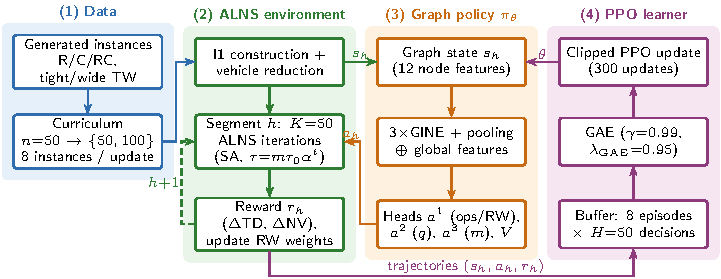
\includegraphics[width=0.62\linewidth]{framework_compact.pdf}
\caption{Training framework of \sgalns{}: generated instances (1) feed complete ALNS
episodes split into segments of $K=50$ iterations (2); before each segment the graph
policy maps the state $s_h$ to an action $a_h$ (3); PPO updates $\theta$ from 8 parallel
episodes (4). Algorithm~\ref{alg:sg} details one episode.}\label{fig:framework}
\end{widefigure}

\para{VRPTW}
Customers $i\in\{1,\dots,n\}$ have demand $d_i$, service time $\sigma_i$ and a hard
time window $[e_i,l_i]$; identical vehicles of capacity $Q$ start and end at depot $0$,
and travel times equal unrounded Euclidean distances $c_{ij}$. Service at $i$ starts at
$b_i=\max\{e_i,\,b_p+\sigma_p+c_{pi}\}\le l_i$, where $p$ is the predecessor of $i$.
As is customary, we minimise the number of vehicles NV, then the total distance TD,
via $f=10^4\,\mathrm{NV}+\mathrm{TD}$; all solutions are re-checked by an independent
feasibility checker.

\para{Underlying ALNS}
All methods share the same ALNS: Solomon's I1 construction~\cite{solomon1987}, a
vehicle-reduction phase of $10n$ iterations~\cite{ropke2006alns}, and a main phase of
$T$ destroy--repair iterations with SA acceptance ($\tau_0$ accepts a deterioration of 5\% of
the initial distance with probability 0.5; $\tau_t=\tau_0\alpha^t$ with $\alpha=0.01^{1/T}$);
a repair that cannot reinsert all customers is discarded. The portfolio
has six destroy operators (random, worst, Shaw, string, route and waiting-time) and
three repair operators (greedy, regret-3 and noisy greedy). Insertion feasibility is
checked in $O(1)$ per position with forward time slack~\cite{savelsbergh1992}, in
Numba kernels. After each segment (100 iterations in \Rw{}, $K$ inside \sgalns{}), RW
updates the weight of operator $o$ as $w_o\leftarrow\max\{(1-\rho)w_o+\rho\,\psi_o/u_o,10^{-3}\}$,
where $\psi_o$ is the total score of $o$ in the segment (33, 9 or 13 per use) and $u_o$
its number of uses ($\psi_o/u_o=0$ if $u_o=0$), with $\rho=0.1$; the normalised weights give
the destroy and repair distributions $(p_D,p_R)=\mathrm{RW}(\vec w)$; the destroy scale is drawn as
$q\sim\mathcal U[0.05n,0.30n]$.

\para{Segment-level MDP}
An episode is one complete main phase, split into $H=T/K$ segments ($K=50$). At the
start of each segment, the agent observes the state $s_h$ and selects a factorised
action $a_h=(a^1,a^2,a^3)$. The component $a^1\in\{0,\dots,18\}$ selects either a
\emph{lead} destroy--repair pair, used with probability 0.7 while the other operators
share the remaining probability uniformly, or ($a^1=18$) the current RW distribution,
whose weights keep being updated; this defines $(p_D,p_R)$. The component $a^2$ sets the
destroy range $\mathcal Q$: $q=\kappa n$ with $\kappa\in\{5,10,20,30\}\%$ or the
default $q\sim\mathcal U[5,30]\%\,n$, and $a^3$
selects a deviation $m\in\{0.3,1,3\}$ \emph{around} the cooling schedule,
$\tau=m\tau_0\alpha^t$. The action $(18,\text{default},1)$ reproduces \Rw{}; we call
this action space \emph{expert-inclusive}, in the spirit of DAC policies that select
among existing heuristics~\cite{speck2021dac}. A headroom study on generated instances,
run before training, motivates it: no fixed lead pair or destroy scale dominates RW
(Table~S4). The reward
\begin{equation}\label{eq:reward}
r_h = 100\,\frac{\mathrm{TD}^\star_{h-1}-\mathrm{TD}^\star_h}{\mathrm{TD}^\star_0}
     +\lambda\,(\mathrm{NV}^\star_{h-1}-\mathrm{NV}^\star_h),\qquad \lambda=5,
\end{equation}
uses the best solution $x^\star$ after each segment; since consecutive terms cancel,
the undiscounted return of an episode equals the final hierarchical improvement (with
the discount $\gamma=0.99$ used in training, early improvements weigh slightly more).
Unlike $f$, which orders all our solutions lexicographically (supplement), the reward
trades one vehicle against 5\% of the initial distance; it is a shaping choice, and we
test its sensitivity to $\lambda$ (\Sect~\ref{sec:collapse}).

\para{State and policy}
The state graph contains the 10 nearest-neighbour arcs of each node and the arcs of the
incumbent. Each node has 6 static features (coordinates, demand, time window and
service time) and 6 dynamic ones (waiting time, slack, forward time slack, load ratio,
route position and a routed flag), all scaled to $[0,1]$ as detailed in the
supplement. A global vector holds the progress $t/T$, the
temperature ratio $\tau/\tau_0$, a stagnation counter, the gaps of the current and
initial solutions to the best one, the fleet ratio and the operators' success rates in
the last segment. Three residual graph isomorphism layers with edge features
(GINE)~\cite{hu2020gine} of width 64, followed by mean and max pooling, feed three
conditionally independent categorical heads, so that $\log\pi(a\mid s)=\sum_k\log
\pi_k(a^k\mid s)$, and a value head (\tParams{} parameters). Output biases are
initialised to favour the expert action, so that learning starts near \Rw{} (a neutral
initialisation is tested in \Sect~\ref{sec:collapse}).


\begin{algorithm}[t]
\caption{\sgalns{}: one episode (actions sampled in training, greedy at deployment)}\label{alg:sg}
\KwIn{instance $I$, policy $\pi_\theta$, segment length $K$, budget $T$}
\KwOut{best solution $x^\star$; trajectory $(s_h,a_h,r_h)_{h=1}^{H}$}
$x\leftarrow\mathrm{VehicleReduction}(\mathrm{SolomonI1}(I))$\;
$x^\star\leftarrow x$; $\vec w\leftarrow\vec 1$; $t\leftarrow0$; $H\leftarrow T/K$\;
\For(\tcp*[f]{one decision per segment}){$h=1,\dots,H$}{
  $s_h\leftarrow\mathrm{GraphState}(x,x^\star,t/T,\tau/\tau_0,\text{success rates})$\;
  $a_h=(a^1,a^2,a^3)\sim\pi_\theta(\cdot\mid s_h)$\;
  \lIf{$a^1=18$}{$(p_D,p_R)\leftarrow\mathrm{RW}(\vec w)$}
  \lElse{$(p_D,p_R)\leftarrow$ lead pair $a^1$ w.p.\ 0.7}
  $\mathcal Q\leftarrow$ destroy range of $a^2$; $m\leftarrow m(a^3)$\;
  \For{$k=1,\dots,K$}{
    $\tau\leftarrow m\,\tau_0\alpha^{t}$; $o_D\sim p_D$; $o_R\sim p_R$; $q\sim\mathcal Q$\;
    $x'\leftarrow o_R(o_D(x,q))$; $t\leftarrow t+1$\;
    \lIf{$f(x')<f(x^\star)$}{$x^\star\leftarrow x'$}
    \lIf{$\mathrm{AcceptSA}(x',x,\tau)$}{$x\leftarrow x'$}
  }
  $r_h\leftarrow$ Eq.~\eqref{eq:reward}; update $\vec w$ from the segment's scores\;
}
\Return $x^\star$ and $(s_h,a_h,r_h)_{h=1}^{H}$\;
\end{algorithm}


\para{Training (Fig.~\ref{fig:framework})}
Each of 300 PPO~\cite{schulman2017ppo} updates runs Algorithm~\ref{alg:sg} with
$T=2{,}500$ on 8 generated instances in parallel and uses generalised advantage
estimation (GAE)~\cite{schulman2016gae} ($\gamma=0.99$, $\lambda_{\mathrm{GAE}}=0.95$,
clip 0.2, Adam with learning rate $3\cdot10^{-4}$, entropy coefficient annealed from
0.01 to 0.001). Instances follow Solomon's design, with $n=50$ for the first 40\% of
the updates and $n\in\{50,100\}$ afterwards. No benchmark instance is used for training
or model selection. Training runs are complete but shorter than at deployment
($T=2{,}500$ vs.\ $5{,}000$): as $t/T$ and the cooling schedule are normalised by $T$, the
policy sees the same relative trajectory, yet its advantage over RW appears only after
2{,}500 iterations (Fig.~\ref{fig:analysis}a). We evaluate the final checkpoint of
\rseedN{} training seeds (seed~0,
used for all ablations, was designated beforehand). One training run takes \tTrainMin{}
minutes on 8 cores.

\para{Context-aware variant (\sgc{})}
\sgalns{} observes neither $n$ nor $T$, so it cannot condition $q$ on the instance size.
\sgc{} appends $n/200$ and $T/5{,}000$ to the global vector and is trained on
$n\in\{50,100,200\}$ with $T\in\{1{,}000,2{,}500,5{,}000\}$ drawn per update
(\tCtxMin{} minutes), a setting that favours instance-dependent behaviour.
